\documentclass[times, utf8, zavrsni]{fer}
\usepackage{booktabs}
\usepackage{listings}
\usepackage{xcolor}
\usepackage{graphicx}
\graphicspath{ {./notes/screenshots/} }

\colorlet{punct}{red!60!black}
\definecolor{background}{HTML}{EEEEEE}
\definecolor{delim}{RGB}{20,105,176}
\colorlet{numb}{black!60!black}

\lstdefinelanguage{json}{
    basicstyle=\normalfont\ttfamily,
    numbers=left,
    numberstyle=\scriptsize,
    stepnumber=1,
    numbersep=8pt,
    showstringspaces=false,
    breaklines=true,
    frame=lines,
    backgroundcolor=\color{background},
    literate=
     *{0}{{{\color{numb}0}}}{1}
      {1}{{{\color{numb}1}}}{1}
      {2}{{{\color{numb}2}}}{1}
      {3}{{{\color{numb}3}}}{1}
      {4}{{{\color{numb}4}}}{1}
      {5}{{{\color{numb}5}}}{1}
      {6}{{{\color{numb}6}}}{1}
      {7}{{{\color{numb}7}}}{1}
      {8}{{{\color{numb}8}}}{1}
      {9}{{{\color{numb}9}}}{1}
      {:}{{{\color{punct}{:}}}}{1}
      {,}{{{\color{punct}{,}}}}{1}
      {\{}{{{\color{delim}{\{}}}}{1}
      {\}}{{{\color{delim}{\}}}}}{1}
      {[}{{{\color{delim}{[}}}}{1}
      {]}{{{\color{delim}{]}}}}{1},
}
\lstset{
  language=bash,
  basicstyle=\ttfamily,
  breaklines=true,
  showstringspaces=false,
  numbers=left,
  stepnumber=1,
  numbersep=8pt,
  frame=lines,
  backgroundcolor=\color{background},
  numberstyle=\scriptsize
}

\begin{document}

% TODO: Navedite broj rada.
\thesisnumber{000}

% TODO: Navedite naslov rada.
\title{Usporedba performanci Ethereum raspodijeljene knjige na raznorodnom sklopovlju}

% TODO: Navedite vaše ime i prezime.
\author{Jakov Buratović}

\maketitle

% Ispis stranice s napomenom o umetanju izvornika rada. Uklonite naredbu \izvornik ako želite izbaciti tu stranicu.
\izvornik

% Dodavanje zahvale ili prazne stranice. Ako ne želite dodati zahvalu, naredbu ostavite radi prazne stranice.
\zahvala{Zahvaljujem se mentoru doc. dr. sc. Igoru Čavraku na podršci i pomoći pri izradi ovog rada.\\
Zahvaljujem se i kolegi Ediju Sinovčiću koji se već dulje vrijeme bavi razvojem programskih rješenja
koji koriste tehnologiju distribuirane knjige te mi je mogao odgovoriti i riješiti sve moje nedoumice.\\
}

\tableofcontents

\chapter{Uvod}
Ethereum mnogi znaju kao jednu od najpopularnijih kriptovaluta. Iako je to točno, Ethereum je mnogo
više od same digitalne valute. To je programska potpora raspodijeljena na mreži računala na kojima je
moguće razmjenjivati podatke i pokretati računalne programe bez centralnog poslužitelja. 
Podaci se repliciraju na svaki čvor u mreži. Određenim algoritmima konsenzusa se osigurava 
nepromjenjivost i pouzdanost. 
To omogućuje da mreža bude potpuno javna i sigurna. Posebnost je što svatko može koristiti
mrežu i objavljivati sadržaj bez ikakvih posebnih dozvola. \\ Za razliku od Bitcoina
i mnogih drugih implementacija tehnologije distribuirane knjige koji nude mogućnost pohrane podataka
bez centralnog poslužitelja, Ethereum mreža omogućuje i izvođenje programskog koda u obliku pametnih ugovora.\\
U ovom radu je prikazano kako se može pokrenuti privatna mreža na različitom sklopovlju s naglaskom
na ispitivanje najnižih zahtjeva sklopovlja. Dodatno, prikazat ću proces obavljanja transakcija
i izvođenja programskog koda na čvorovima uz prigodni prikaz sa sučeljem u jednostavnoj web aplikaciji.\\
U prvom poglavlju ovog rada, objasnit će se osnove tehnologije distribuirane knjige i njene primjene.\\
Nakon toga će biti poglavlje usmjereno na Ethereum kao implementaciju navedene tehnologije te prikaz
i opis njegovih algoritama konsenzusa. \\
Treće poglavlje je zaduženo za detaljan postupak kreiranja privatne mreže na raznorodnom sklopovlju
s različitim operativnim sustavima. \\
U posljednjem poglavlju je na prethodno kreiranu mrežu dodan grafički prikaz aktivnosti mreže i transakcija
u jednostavnoj web aplikaciji. 

\chapter{Tehnologija glavne raspodijeljene knjige}
U nastavku ćemo tehnologiju glavne raspodijeljenje knjige (engl. \emph{Distributed Ledger Technology})
 referencirati kraće po kratici engleskog naziva, odnosno DLT. \\ 
DLT i blockchain se češto poistovjećuju no to nije u potpunosti ispravno. Bitno je znati da je 
svaki blockchain DLT s određenim pravilima konsenzusa.
DLT je baza podataka repliciranog sadržaja na svakom čvoru \emph{peer-to-peer} mreže. Svaki čvor
mora sadržavati identičnu kopiju kompletnog sadržaja baze podataka i konstantno se ažurira sa susjednim
čvorovima. \\
Kod blockchaina se te promjene zapisuju u obliku transakcije u blokove koji formiraju neprekidan lanac.
Odatle dolazi i sam naziv tehnologije. Prije nego što se novi blok transakcija poveže u postojeći lanac
blokova, on mora biti potvrđen od većine čvorova prema poznatim pravilima konsenzusa koji se koristi
u toj implementaciji mreže. Nakon što je blok povezan, sve transakcije zabilježene ostaju zauvijek i
šanse za maliciozne izmjene su vrlo malene. Više o mogućim napadima će biti opisano u nastavku jer
se razlikuju za ovisno o implementaciji. \\
Bitcoin je najpoznatiji primjer primjene blockchaina u široj populaciji. Njegova mreža je aktivna 
od siječnja 2009. godine kada je Satoshi Nakamoto potvrdio prvi blok (engl. \emph{genesis}).
Još uvijek nije poznato tko je Satoshi Nakamoto i je li to uopće stvarna osoba ili naziv za grupu
ljudi koji su sudjelovali u tazvoju bitcoina. Problem koji bitcoin pokušava riješiti je centraliziranost
ekonomskog sustava i plaćanja. Svaka transkacija u trenutnom sustavu mora proći kroz centralno sjedište,
odnosno banku. To znači da korisnici moraju vjerovati centralnom sjedištu da će provesti transakcije
kako korisnik želi i da se neće ponašati maliciozno. Također, korisnici moraju vjerovati u sigurnost
centralnog sjedišta i mogućnost zaštite od napada od treće strane. \\
Za takav način je potreban velik broj ljudi, novca i kontrole što dovodi dodatna ograničenja kao što 
su čekanje na potvrdu transakcije dulje vrijeme, nemogućnost obavljanja transakcija vikendom i praćenje
toka novca. \\
Bitcoin te probleme rješava na način da izbacuje centralno sjedište i umjesto njega koristi \emph{Proof of Work}
pravila konsenzusa koja osiguravaju pouzdanost bez povjerenja. \\
Nakon bitcoina su se pojavili mnogi \emph{forkovi} s manjim ili većim promjenama, obično u veličini
samih blokova ili brzini potrvrđivanja istih. Oni su obilježili prvu generaciju kriptovaluta. \\
2013. godine ruski programer Vitalik Buterin predlaže Ethereum, novu javnu platformu koja koristi 
dorađeno izdanje Nakamotovog \emph{PoW} konsenzusnog algoritma. Posebnost Ethereuma jest da on nije
samo raspodijeljena platforma za transakcije, već raspodijeljeni virtualni stroj (engl. \emph{Ethereum Virtual Machine -EVM})
 koji može izvoditi kod poznat pod nazivom pametni ugovor (engl. \emph{smart contract}). \\



\chapter{Proof of Authority algoritam}

\chapter{PoA mreža na raznovrsnom sklopovlju}
Glavni zadatak ovog završnog rada bio je postaviti vlastitu mrežu koristeći Ethereum platformu na raznorodnom sklopovlju
te provjeriti koliko su visoki zahtjevi jedne takve mreže na hardver. Osim same mreže, dodane su još neke osnovne funkcionalnosti
kako bi se što ovi laboratorijski uvjeti što više približili pravom svijetu te nam ponudili kvalitetnije rezultate. Tako recimo
imamo postavljen pretražitelj blokova (engl. \emph{Block explorer}) koji u realnom vremenu prikazuje putem web aplikacije
trenutni blok i transakcije koje su se provele u tom bloku. Moguće je i pretraživati starije blokove putem njega. \\
Osim pretražitelja blokova, dodana je i još jedna web aplikacija koja nudi podatke o opterećenosti pojedinog čvora u mreži
što je korisno za ovaj završni rad jer jednostavno možemo usporediti opterećenost na raznorodnom sklopovlju. \\
Posljednja funkcionalnost jest zapravo podizanje (engl. \emph{deployment}) najjednostavnijeg pametnog ugovora kako bismo
zapravo mogli vidjeti samu komunikaciju između čvorova i izvođenje programskog koda.

\section{Sklopovlje i programska podrška}
Ono što čini ovaj sustav zanimljivim i pristupačnim širokoj populaciji je mogućnost sudjelovanja u distribuiranoj mreži s vrlo
različitim sklopovljem. To znači da korisnici u većini slučajeva neće morati ulagati novac u novi hardver.\\ U ovom radu su korištena
tri uređaja s ARM procesorima, jedno prijenosno računalo s Intel 64 bitnim procesorom i stolno računalo s AMD 64 bitnim procesorom.
\subsection{Cubieboard2}
Cubieboard2 jest jednostavno računalo (engl. \emph{single-board computer}) kompanije Cubietech. Ovo računalo jest otvoreno
što znači da su svi podaci o sklopovlju dostupni javno. Cubieboard2 je njihov drugi proizvod, izravni nasljednik originalnog Cubieboarda.\\
Pogoni ga Allwinner A20 čipset kojeg čini dvojezgreni Cortex-A7 procesor takta 1 GHz s Mali400 grafičkim sklopom. 
Na ploči je integrirana radna memorija DDR3 kapaciteta 1 GB na taktu 480 MHz i memorija za pohranu od 4 GB. Memorija za pohranu je 
proširiva microSD memorijskom karticom.
Ne postoji ugrađen modul za bežičnu povezivost putem Wifi-a pa je korišten Ethernet ulaz propusnosti 10M/100M. \\
Ovo računalo je moguće napajati putem USB micro sučelja ili DC 5V ulaza. \\
Obzirom da je Cortex-A7 ARM procesor postoje razne mogućnosti kad je u pitanju odabir operativni sustav. Tvornički dolazi
Android da unutarnjoj memoriji od 4 GB što nije odgovaralo potrebama ovog rada pa je bilo potrebno pronaći odgovarajuću distribuciju
Linux operativnog sustava.\\ Odličan izbor se pokazala distribucija armbian koja je ponudila minimalnu instalaciju operativnog sustava
za ovo računalo baziranu na Debian Linuxu. Dolazi s ažurnom verzijom Linux kernela 5.4 što znači da sa strane programske podrške
postoje dobri uvjeti. \\
Nakon instalacije operativnog sustava, ažurirani su svi paketi, postavljena je statična IP adresa kako bi se bilo moguće udaljeno
povezati na računalo putem SSH protokola. 
\subsection{Raspberry Pi 1 model B}
Raspberry Pi je najraširenije jednostavno računalo. Model 1B jest prva generacija iz 2012. godine koja po današnjim standardima
donosi vrlo ograničene performance. \\
Ovo računalo je dizajnirano oko Broadcom BCM2835 sustava na čipu (engl. \emph{SoC}) koji sadrži ARM1176JZF-S procesor na ARMv6
arhitekturi i radnom taktu od 700 MHz. Usko grlo jest 256 MB radne memorije od kojih je samo 192 MB dostupno procesoru a ostatak je
rezerviran za obradu multimedijskog sadržaja. Ne postoji nikakva ugrađena memorija za pohranu nego sva pohrana ide na SD karicu.
Kao i kod Cubieboard2 računala, niti ovdje ne postoji ugrađeni Wifi modul pa su mogućnosti svedene na Ethernet ulaz ili USB
adapter za Wifi. Računalo se napaja putem USB micro sučelja.\\
Obzirom da je Raspberry Pi vrlo raširen, operativni sustav je vrlo lako dostupan i redovno održavan. Korišten je službeni
Raspbian operativni sustav koji je baziran na Debian Linux distribuciji. Raspbian dolazi u dvije varijante, s grafičkim sučeljem
i bez njega (engl. \emph{headless}). Za ovaj rad je primjerenije odabrati opciju bez grafičkog sučelja kako ne bismo trošili
resurse nepotrebno na prikaz slike i razne dodatne procese koji su porenuti s grafičkim sučeljem. \\
Nakon instalacije Raspbiana, paketi su ažurirani i kao i kod Cubieboard2 računala, postavljena je statična IP adresa i upaljen SSH
servis. \\
Već prilikom ovog postavljanja se vidi da je u odnosu na Cubieboard2 ovo računalo dosta nižih performanci.
\subsection{Raspberry Pi 3 model B}
Ovaj model je najranije izdanje treće generacije Raspberry Pi računala. Sklopovljem je mnogo bliži Cubieboard2 računalu nego
svom predhodniku prve generacije. \\
Pogoni ga četverojezgreni Broadcom BCM2837 64 bitni procesor radnog takta 1,2 GHz. Baziran je na armhf arhitekturi.
BCM2837 ima ugrađeni modul za bežičnu povezivost putem Wifi-a i Bluetooth-a. Na ploči je 1 GB radne memorije i kao i njegov prethodnik
nema memoriju za pohranu na ploči nego za to koristi microSD karticu. Napaja se putem USB Micro sučelja. \\
Ponovno je odabir operativng sustava raznovrstan zbog raširene arhitekture procesora no većina korisnika koristi službeni 
Raspbian. Odabrana je opcija bez grafičkog sučelja te su provedeni koraci kao i za prethodna dva računala. \\
Postavljanje sustava i postavki je značajno brže nego na Raspberry Pi 1 modelu što je očekivano obzirom na sklopovlje.
\subsection{Prijenosno i stolno računalo}
Prijenosno računalo kao i stolno računalo je u raširenijoj uporabi u kućanstvima i upravo takvim sklopovljem se može
najvjernije prikazati kako gotovo bilo tko može sudjelovati u jednoj distribuiranoj mreži na Ethereum platformi. \\
Sklopovlje na korištenim računalima u ovom radu ne spada među najmoderniji sloj trenutno dostupnog sklopovlja no i dalje
je mnogo snažnije nego na single-board računalima. \\
Prijenosno računalo pogoni Intel Pentium četverojezgreni procesor N3530 čiji radni takt seže do maksimalnih 2,58 GHz.
Ugrađeno je 8 GB radne memorije i za pohranu se koristi SSD kapaciteta 500 GB. Ovaj procesor je 64 bitne arhitekture.
Kao i većina prijenosnih računala danas i ovo posjeduje ugrađenu mrežnu karticu koja nudi bežićnu povezivost. \\
Stolno računalo pogoni AMD Phenom II X4 925 procesor čiji je takt podignut na 3,4 GHz. Arhitekture procesora je 64 bitna.
Također ima 8 GB radne memorije na taktu 800 MHz. Podaci se pohranjuju na SSD od 250 GB. \\
Računalo je povezano putem Ethernet sučelja na usmjeritelj (engl. \emph{Router}). \\
Na prijenosnom računalu je instaliran Xubuntu 20 operativni sustav dok je na stolnom računalu instaliran Ubuntu 19.10.
Oba operativna sustava su redovno ažurirana i imaju postavljene statične IP adrese.
\section{Geth privatna mreža}
Geth je službena implementacija Ethereum protocola u programskom jeziku Go. Izvorni kod je javno dostupan na Github platformi. \\
Postavljanje je vrlo dobro opisano u službenoj dokumentaciji. Potrebno ga je instalirati ili pokretati iz docker kontejnera. 
Za ovaj rad je odabrana klasična instalacija zbog boljih performanci i smanjenja općih troškova (engl. \emph{overhead}).
Obzirom da svaki uređaj koji je korišten pokreće neku distribuciju linuxa temeljenu na Debianu, instalacija je jednostavna
i već su dostupne unaprijed izgrađene binarne datoteke za ARM i amd64 arhitekture. Potrebno je odabrati odgovarajući paket na
stranici za preuzimanje \url{https://geth.ethereum.org/downloads/}.\\ Za Cubieboard2 i Raspberry Pi računala je odabran paket
preveden za ARMv7 arhitekturu dok je za oba računala odabran paket preved za 64 bitnu arhitekturu. \\
Na Debian baziranim operativnim sustavima je također moguće instalirati Geth putem \emph{apt} repozitorija. \\
\subsection{Generiranje novčanika i konfiguracijska datoteka}
Da bismo izgradili privatnu Ethereum mrežu potrebno je inicijalizirati novčanik (engl \emph{wallet}) za svaki čvor. Taj novčanik
će biti identifikator pojedinog čvora u mreži. \\
Potrebno je kreirati novi direktorij u kojem će se nalaziti sve potrebne datoteke za Geth i naredbom generirati u nju novi novčanik.

\begin{lstlisting}
    $ mkdir node
    $ geth --datadir node/ account new
\end{lstlisting}

Nakon izvođenja naredbi, Geth će tražiti korisnika da unese lozinku kojom će biti zaštićen novčanik.

\begin{lstlisting}
INFO [05-19|20:01:00.571] Maximum peer count ETH=50 LES=0 total=50
INFO [05-19|20:01:00.580] Smartcard socket not found, disabling err="stat /run/pcscd/pcscd.comm: no such file or directory"
Your new account is locked with a password. Please give a password. Do not forget this password.
Password: 
Repeat password: 
Your new key was generated
Public address of the key: 0xBC60333862ccdB3E515d9b274834552ce24739eE
Path of the secret key file: node/keystore/UTC--2020-05-19T18-01-09.785462468Z--bc60333862ccdb3e515d9b274834552ce24739ee
- You can share your public address with anyone. Others need it to interact with you.
- You must NEVER share the secret key with anyone! The key controls access to your funds!
- You must BACKUP your key file! Without the key, it's impossible to access account funds!
- You must REMEMBER your password! Without the password, it's impossible to decrypt the key!
\end{lstlisting}

Korisnik dobiva upute kako ne smije dijeliti tajni ključ zbog toga što vrijedi da svatko tko posjeduje tajni ključ novčanika
posjeduje i sadržaj odovarajućeg novčanika. U ovom primjeru to nije problem jer se balans svakog novčanika postavlja u \emph(genesis)
datoteci koju će učitati svaki čvor prije uključivanja u mrežu. Ta datoteka govori čvoru na koju mrežu da se spoji putem identifikatora
mreže, daje mu upute o učestalosti kreiranja novih blokova, navodi koji je algoritam konsenzusa korišten i postavlja inicijalni balans
odabranim novčanicima. Kako gradimo privatnu testnu mrežu, dobra je praksa postaviti svakom čvoru dovoljno \emph{Ethera} kako bismo
prilikom testiranja mogli nesmetano obavljati transakcije i komunicirati s drugim čvorovima. \\
U nastavku je prikazana \emph{genesis.json} datoteka koja je korištena u ovom primjeru.

\begin{lstlisting}[language=json,firstnumber=1]
    {
  "config": {
    "chainId": 15316,
    "homesteadBlock": 0,
    "eip150Block": 0,
    "eip150Hash": "0x0000000000000000000000000000000000000000000000000000000000000000",
    "eip155Block": 0,
    "eip158Block": 0,
    "byzantiumBlock": 0,
    "constantinopleBlock": 0,
    "petersburgBlock": 0,
    "istanbulBlock": 0,
    "clique": {
      "period": 15,
      "epoch": 30000
    }
  },
  "nonce": "0x0",
  "timestamp": "0x5ec4241f",
  "extraData": "0x00000000000000000000000000000000000000000000000000000000000000006e088347443a6c361f281e533afc805c4f1900b5968245a9bd3afa193995bd01c055d7aa4597b3e8ad59da52e58e82799bfb7cc360f49eed872bc586bc60333862ccdb3e515d9b274834552ce24739eed907a7f584cc815ef8da06320feb8206107ee2700000000000000000000000000000000000000000000000000000000000000000000000000000000000000000000000000000000000000000000000000000000000",
  "gasLimit": "0x47b760",
  "difficulty": "0x1",
  "mixHash": "0x0000000000000000000000000000000000000000000000000000000000000000",
  "coinbase": "0x0000000000000000000000000000000000000000",
  "alloc": {
    "6e088347443a6c361f281e533afc805c4f1900b5": {
      "balance": "0x200000000000000000000000000000000000000000000000000000000000000"
    },
    "968245a9bd3afa193995bd01c055d7aa4597b3e8": {
      "balance": "0x200000000000000000000000000000000000000000000000000000000000000"
    },
    "ad59da52e58e82799bfb7cc360f49eed872bc586": {
      "balance": "0x200000000000000000000000000000000000000000000000000000000000000"
    },
    "bc60333862ccdb3e515d9b274834552ce24739ee": {
      "balance": "0x200000000000000000000000000000000000000000000000000000000000000"
    },
    "d907a7f584cc815ef8da06320feb8206107ee270": {
      "balance": "0x200000000000000000000000000000000000000000000000000000000000000"
    }
  },
  "number": "0x0",
  "gasUsed": "0x0",
  "parentHash": "0x0000000000000000000000000000000000000000000000000000000000000000"
}
\end{lstlisting}

U "config" odjeljku se definira identifikator mreže i algoritam konsenzusa. Ovdje je to \emph{clique}. U njegovim opcijama je namješten
period na 15 sekundi i \emph{epoch} koji govori nakon kojeg bloka se kreira točka (engl. \emph{checkpoint}) nakon koje će čvorovi moći
uskladiti svoje stanje bez da provjeravaju povijest od prvog bloka, odnosno \emph{genesis} bloka. Dovoljno je očitati stanje na \emph{checkpointu}
što donosi velika poboljšanja u performancama uz određeni kompromis u sigurnosti algoritma. \\
Osim tih polja, za \emph{Proof of Authority} je jedino još važno u polje "alloc" dodati sve čvorove kojima će biti dozvoljeno potvrđivati
nove generirane blokove (engl. \emph{sealing blocks}). Redom adrese navedene su adrese novčanika Raspberry Pi 3 pločice, AMD stolnog računala, Intel prijenosnog
računala i poslijednje dvije su adrese dvije različite Cubieboard2 pločice. \\
\subsection{Inicijalizacija čvorova}
Kako bi čvorovi bili ispravno konfigurirani za povezivanje u istu mrežu s jednakim uputama o vremenu kreiranja blokova i ostalih konfiguracijskih
parametara, potrebno je svaki čvor inicijalizirati istom \emph{genesis.json} datotekom. 

\begin{lstlisting}
$ geth --datadir node/ init genesis.json
\end{lstlisting}
U ovom trenutku je svaki čvor spreman uključiti se u mrežu.
\subsection{Detekcija čvorova}
Da bi mreža bila valjana i funkcionalna, potrebno je da čvorovi budu povezani i da se vide međusobno.
Kako bi se to osiguralo koristi se jedan dodatni čvor koji neće sudjelovati u potvrđivanju i kreiranju novih blokova
nego će samo listu IP adresa svih dolaznih konekcija čvorova slati nazad čvorovima. Na taj način će čvorovi znati s kim komunicirati.
Ta uloga je pridijeljena Raspberry Pi pločici prve generacije jer su sklopovski zahtjevi mnogo niži nego za klasični čvor.
Ovaj čvor zovemo \emph{bootnode}. \\
Sljedećim naredbama generiramo ključ te pokrećemo \emph{bootnode} na portu 30310. Dodana je opcija -verbosity 9 kako bismo vidjeli
detaljan ispis događaja u konzoli. \\

\begin{lstlisting}
    $ bootnode -genkey boot.key
    $ bootnode -nodekey boot.key -verbosity 9 -addr 192.168.1.13:30310
\end{lstlisting}

\emph{Bootnode} ispisuje svoj identifikator koji treba pospremiti i čeka na čvorove.
\subsection{Pokretanje geth procesa na čvorovima}
Nakon što su svi prethodni koraci uspješno obavljeni preostaje pokrenuti geth čvor na svakom uređaju. Dovoljna je jedna naredba
kojom se zadaje identifikator \emph{bootnodea} i mreže i adresa novčanika koja će predstavljati čvor. 

\begin{lstlisting}
  $ geth --datadir node/ --syncmode 'full' --bootnodes 'enode://<identifikator>@192.168.1.13:0?discport=30310' --networkid 15316 --gasprice '1' -unlock '0xBC60333862ccdB3E515d9b274834552ce24739eE' --allow-insecure-unlock --mine
\end{lstlisting}


\begin{figure}[h]
  \caption{Ispis nakon pokretanja geth procesa}
  \centering
  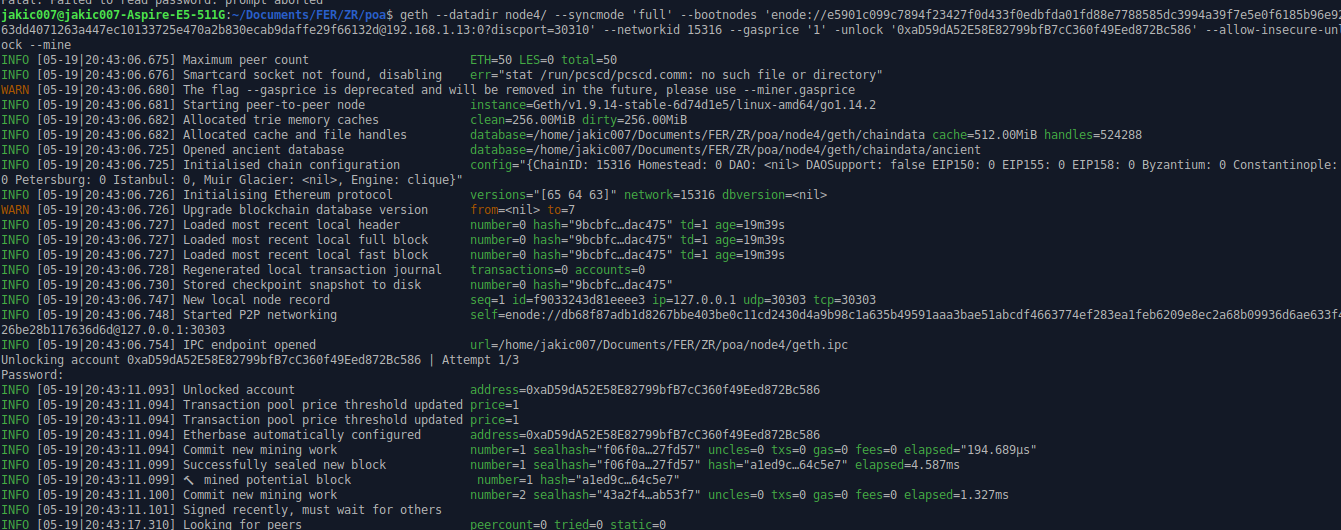
\includegraphics[width=\textwidth]{nodeStart.png}
\end{figure}

Iz ispisa se može vidjeti kako je nakon upisane lozinke za otključavanje novčanika pokrenuto rudarenje, odnosno kreiranje blokova.
Kao što je već objašnjeno detaljnije u prethodnom poglavlju, potrebno je imati (N/2)+1 čvorova \emph{online} kako bi se blokovi
kontinuirano stvarali gdje je N broj adresa navedenih u \emph{genesis.json} datoteci. U slučaju da neki čvor \emph{ispadne},
blokovi će se stvarati dokle god je dovoljno aktivnih čvorova. Kad se čvor ponovno poveže, on će uskladiti svoje stanje
s ostalima kako bi povijest bila svugdje jedinstvena. \\
Novi blok se generira svako 15 sekundi jer je tako zadano prilikom incijalizacije \emph{genesis.json} datotekom. \\
U isto se vrijeme na \emph{bootnodeu} vide \emph{ping-pong} poruke čvorova što znači da su svi čvorovi uspješno povezani i međusobno
vidljivi.

\begin{figure}[h]
  \caption{Komunikacija čvorova i \emph{bootnodea}}
  \centering
  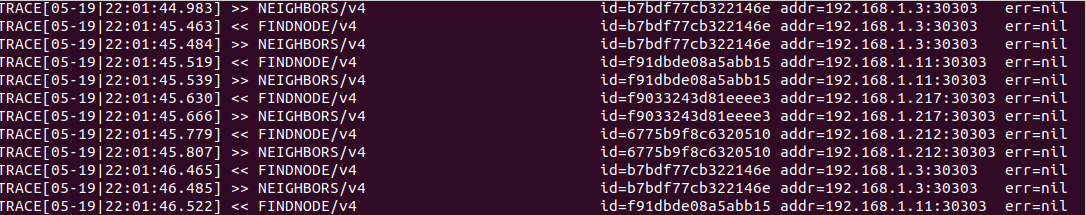
\includegraphics[width=\textwidth]{bootnode.png}
\end{figure}

\pagebreak
\section{Praćenje stanja (engl. \emph{monitoring})}
U prijašnjem odjeljku je pokrenuta potpuno funkcionalna mreža no korisnicima nije jednostavno pratiti stanje gledajući
dnevnike (engl. \emph{logs}) iz komandne linije. Postoji mnogo besplatnih dostupnih i otvorenih alata koji nude jednostavniji
prikaz bitnih podataka u obliku jednostavne web aplikacije koja se povezuje izravno na čvor. Obično se koristi http protokol
ili websocket veza kako bi se podaci dobavljali.
\subsection{Pretražitelj blokova (engl. \emph{block explorer})}
Osnovni dio praćenja stanja je \emph{block explorer}. Pomoću njega se može u realnom vremenu pratiti stanje \emph{blockchaina}
što podrazumijeva prikaz najvišeg trenutnog bloka (engl. \emph{block height}) te pretraživanje i filtriranje transakcija u 
pojedinom bloku. \\
Odabrana je aplikacija \emph{Alethio Ethereum Lite Explorer} zbog svoje jednostavnosti i ažurnosti. To je klijentska
web aplikacija koja se povezuje na bilo koji \emph{Ethereum} čvor koji ima omogućen udaljen poziv procedura (engl. \emph{RPC}). \\
Čvorovi postavljeni u prethodnom dijelu nemaju omogućen udaljen poziv procedura. Da ga omogućili potrebno je zaustaviti geth proces
na odabranom uređaju te ponovno pokrenuti dodavanjem parametara:

\begin{lstlisting}
  --rpc --rpcaddr 'localhost' --rpcport 8545  --rpcapi 'personal,db,eth,net,web3,txpool,miner' --rpccorsdomain "*"
\end{lstlisting}

Ovim postupkom je omogućeno spajanje bilo kojeg servisa s istog računala na naš \emph{geth} proces putem porta 8545 i http protokola.

Postoje dva načina pokretanja ove aplikacije, prevođenjem izvornog koda na vlastitom računalu ili već javno dostupnim
\emph{docker} kontejnerom. Zbog jednostavnosti i niske zahtevnosti, za ovaj projekt je odabran drugi način.
Jedini preduvjet je imati instaliran \emph{docker} klijent na računalu. Nakon toga se sve pokreće jednom naredbom.

\begin{lstlisting}
  $ docker run -p 8080:80 -e APP_NODE_URL="http://localhost:8545" alethio/ethereum-lite-explorer
\end{lstlisting}

\emph{Docker} provjerava postoji li već lokalno dostupna slika te ako ne postoji je dohvaća s \emph{Docker Hub} repozitorija.
Ovim načinom nije potrebno mijenjati konfiguracijsku datoteku već je dovoljno samo dodati varijablu okoline (engl. \emph{environment variable})
koja aplikaciji daje IP adresu i vrata čvora na koji se potrebno spojiti. \\
Parametrom "-p 8080:80" se prosljeđuje \emph{port} 80 unutar kontejnera na \emph{port} 8080 na uređaju na kojem se pokreće kontejner. \\
Utipkavanjem adrese "localhost:8080" u željeni preglednik otvara se aplikacija i prikazuje početni ekran. \\
Blok 47 na slici je prazan, odnosno niti jedna transakcija se nije dogodila u njemu.

\begin{figure}[h]
  \caption{Početni ekran pretražitelja blokova}
  \centering
  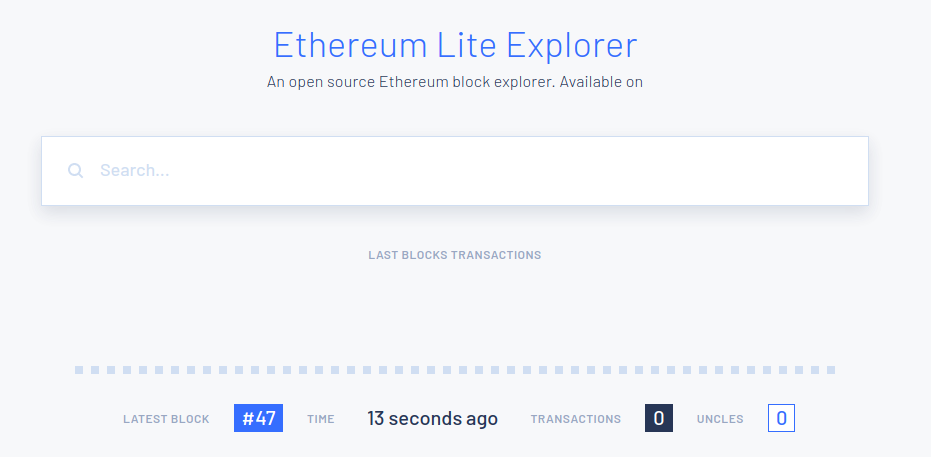
\includegraphics[width=\textwidth]{blockexplorer.png}
\end{figure}

\subsection{Opterećenost čvorova}
Za dobivanje podataka potrebnih za usporedbu performanci na raznorodnom sklopovlju potreban je poseban servis koji će pratiti
opterećenost sklopovlja čvora. Jednako kao i za praćenje stanja blokova, postoji više dostupnih alata. Za ovaj rad je ponovno
odabran \emph{Alethiov} alat \emph{ethstats}. Razlog tome je što je jedini redovno održavan, besplatan i moguće ga je pokrenuti
uz vrlo malo konfiguracije pomoću \emph{docker-composea}. \\
Dovoljno je preuzeti datoteku s poveznice
 \footnote{\url{https://raw.githubusercontent.com/Alethio/ethstats-network-server/master/docker/lite-mode/redis-persistence/docker-compose.yml}} koju 
 treba izmijeniti za ovu konfiguraciju. \\
\emph{Ethstats} se sastoji od više servisa koji čine cjelinu. \emph{Docker-compose} nam olakšava pokretanje te nakon podešavanja
varijabli okruženja unutar \emph{docker-compose.yaml} datoteke moguće je pokrenuti sve servise jednom naredbom.
\begin{lstlisting}
  $ docker-compose up -d
\end{lstlisting}
Time smo pokrenuli \emph{ethstats server}, \emph{dashboard}, \emph{redis} i \emph{deepstream}.
Server pribavlja podatke sa čvorova i sprema ih u \emph{Redis} bazu podataka i istovremeno pruža \emph{dashboardu} i \emph{deepstreamu} koji
su zaduženi za grafički prikaz i analitiku. \\
Pokretanjem prethodne naredbe dobiva se pogreška koja kaže da se server ne može povezati na \emph{ethstats-cli}. \emph{ethstats-cli} 
je odvojeni servis koji se treba pokrenuti na svakom čvoru koji se želi pratiti. On je zaslužan za prikupljanje podataka o iskorištenosti
memorije, procesora i ostalih detalja o sklopovlju. Njegov zatjev je prethodno instaliran \emph{node} verzije novije od 8.11 što se može 
provjeriti naredbom:
\begin{lstlisting}
  $ node -v
\end{lstlisting}
Kad je osigurana odgovarajuća verzija \emph{nodea} moguće je globalno instalirati \emph{ethstats-cli} i pokrenuti naredbama:
\begin{lstlisting}
  $ npm install -g ethstats-cli
  $ ethstats-cli --server-url http://192.168.1.217:3000 -r --account-email jakov.buratovic@fer.hr --node-name pc
\end{lstlisting}
Prvim pokretanjem obavlja se registracija čvora pa je zbog toga unesena adresa e-pošte i proizvoljan naziv čvora. IP adresa u argumentu
"--server-url" jest IP adresa računala na kojem će biti pokrenut \emph{ethstats-server}. U ovom primjeru je to prijenosno računalo. \\
Sada možemo izmijeniti \emph{docker-compose.yaml} datoteku željenim uređivačem teksta. Dovoljno je promijeniti konfiguraciju servisa
\emph{server} na sljedeći način:
\begin{lstlisting}
  server:
    container_name: ethstats-network-server
    image: alethio/ethstats-network-server:latest
    restart: always
    depends_on:
      - deepstream
      - redis
    ports:
      - 127.0.0.1:3000:3000
      - 192.168.1.217:3000:3000
      - 127.0.0.1:3030:3030
      - 127.0.0.1:8888:8888
    environment:
      - NETWORK_ID=15316
      - NETWORK_NAME=dev
\end{lstlisting}

U odnosu na zadanu konfiguraciju, dodano je preusmjeravanje unutarnjeg porta 3000 na vanjsko sučelje računala kako bi ostali uređaji
u lokalnoj mreži mogli vidjeti \emph{ethstats-server} te je izmijenjen identifikator mreže koji je bio postavljen na vrijednost "1" što
označava glavnu Ethereum mrežu \emph{Ethereum mainnet}. Ako ponovno pokrenemo \emph{docker-compose} trebali bismo uspješno biti povezani
na čvorove i posjetom adrese "localhost:80" biti će prikazano sučelje.

\begin{figure}[h]
  \caption{Sučelje \emph{ethstatsa}}
  \centering
  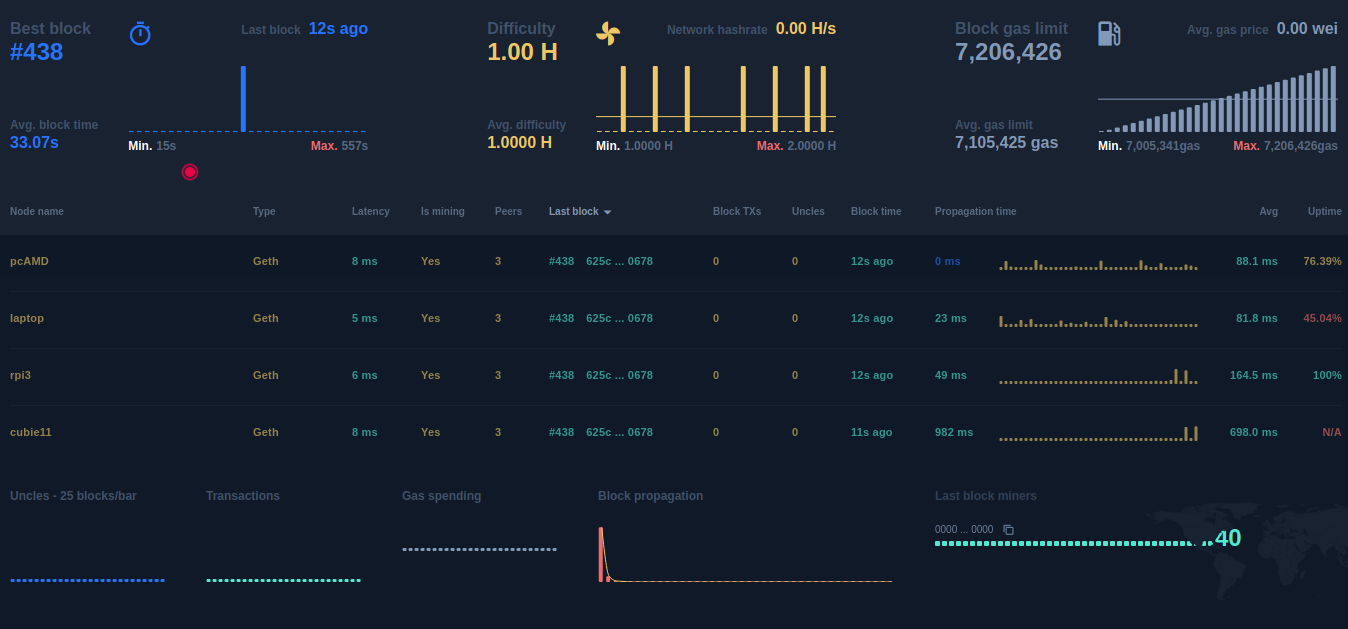
\includegraphics[width=\textwidth]{ethstatsDashboard.png}
\end{figure}

Kao i u \emph{block exploreru} vidljiv je posljednji blok no ovoga puta uz više detalja i podacima za svaki čvor posebno.
Desno od posljednjeg bloka vidimo statistiku o vremenu kreiranju novih blokova. Minimalno vrijeme je 15 sekundi što odgovara konfiguraciji
no maksimalno vrijeme je 557 sekundi što znači da 557 sekundi nije bilo dovoljno povezanih čvorova u mreži i proizvodnja blokova je stala. \\
Ispod vidimo listu svih čvorova s osnovnim podacima kao što su brzina odaziva, broj povezanih čvorova na taj čvor, posljednji blok na pojedinom
čvoru te brzinu propagiranja novog bloka na čvoru. \\
Iz ove liste vidimo da su svi čvorovi sinkronizirani na istom posljednjem bloku što nam govori da je njihovo sklopovlje dovoljno sposobno
pokretati ovakav tip mreže. Veće opterećenje se može postići skraćivanjem vremena kreiranja blokova i izvršavanjem složenih programskih
kodova pametnih ugovora. \\
Za više detalja potrebno je odabrati čvor čime se otvara novi prikaz u kojem vidimo zauzeće procesora i radne memorije u odabranom
vremenskom razdoblju.
\begin{figure}[h]
  \caption{Opterećenost Cubieboard2 pločice}
  \centering
  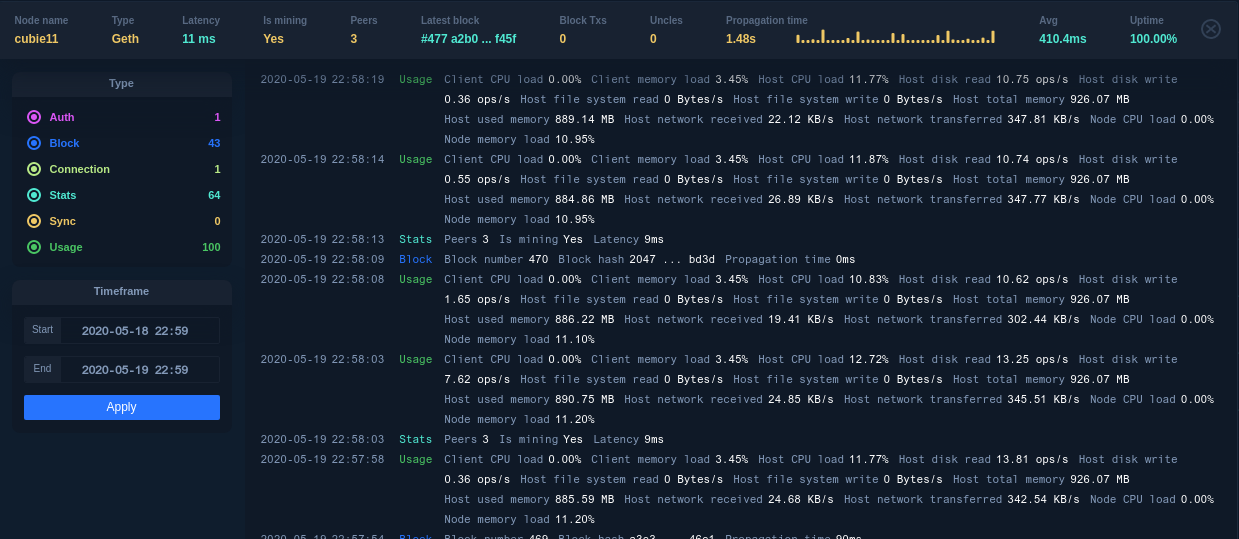
\includegraphics[width=\textwidth]{ethstatsCubie.png}
  \vspace{10in}
\end{figure}

\section{Transakcije i pametni ugovori}



\chapter{Zaključak}
Zaključak.

\bibliography{literatura}

\bibliographystyle{fer}

\begin{sazetak}
Sažetak na hrvatskom jeziku.

\kljucnerijeci{Ključne riječi, odvojene zarezima.}
\end{sazetak}

% TODO: Navedite naslov na engleskom jeziku.
\engtitle{Performance Comparison of the Ethereum Blockchain on Heterogeneous Hardware}
\begin{abstract}
Abstract.

\keywords{Keywords.}
\end{abstract}

\end{document}
